Parmi les nombreuses implémentations des \emph{sous-ensembles flous
  spatialisés} présentées jusqu'ici (\autoref{chap:03}), on retrouve
aussi bien des approches vectorielles
\autocite{Kanjilal2010,Dilo2007,Zoghlami2016} ou raster
\autocite{Bloch1996}, que des approches fondées sur la sélection
d'objets préexistants \autocite{Duraciova2017}. Toutes ont des
avantages et des inconvénients qu'il est nécessaire d'étudier,
d'autant que ses solutions ne conservent pas nécessairement toutes les
qualités du modèle théorique. Par exemple, les approches vectorielles
proposées par \textcite{Kanjilal2010,Zoghlami2016} se basent sur la
discrétisation vectorielle d'un sous-ensemble flou. Ces
implémentations ont donc une précision de représentation qui dépend du
nombre de régions utilisées pour discrétiser le \emph{sous-ensemble
  flou.} Si elles sont au nombre de deux, ces implémentations se
comportent comme les modèles \enquote{exacts} et ne sont pas plus
utilisables que ces derniers. L'augmentation du nombre de vecteurs
permet de régler ce problème et de représenter tout type de
\emph{zones de localisation.}

\tdi{Parler limites vecteurs et sélection}

Chacune de ces deux implémentations permet la construction de
\emph{zones de localisation compatibles} à partir de \emph{relations
  de localisation} non linéaires. En effet, bien qu'elles imposent
toutes deux un échantillonnage des sous-ensembles flous, elles
permettent de rendre des variations non linéaires. De la même manière,
ces deux approches permettent de construire des \emph{zones de
  localisation} dont les limites peuvent être \emph{imprécises} ou
assez précises. Nous proposons de confronter les deux implémentations
qui nous semblent être les plus prometteuses, l'utilisation
\emph{d'alpha-cuts} vectorielles et l'utilisation de rasters.

\subsection{Définition d'un exemple comparatif}

Les implémentations de la \emph{théorie des sous-ensembles flous} à
l'aide d'une approche par \emph{alpha-cuts} ou par raster nous
semblent toutes les deux pertinentes pour notre cas
d'utilisation. Nous proposons donc de les comparer en les utilisant
pour spatialiser un même exemple \autocite{Bunel2019a}. Pour ce faire
nous allons utiliser l'un des \emph{indices de localisation} du
\emph{fil rouge} : \enquote{La victime est située sous une ligne
  électrique 3 brins}. Cet \emph{indice} présente le double avantage
d'être simple à modéliser ---~et donc à comparer~---, tout en
utilisant une \emph{relation de localisation,} décomposable, ce qui
permet de tester également les opérations de fusion inter \emph{zones
  de localisation.}

% Définition de l'aire
Pour faciliter la comparaison de ces deux implémentations, nous nous
sommes focalisés sur une petite partie de la zone du \emph{fil rouge}
(\autoref{fig:fil_rouge}), ce qui nous permet de ne travailler qu'avec
un seul \emph{objet de référence} candidat (\autoref{fig:ZIR_HT}).
Ainsi, pour cet exemple nous ne nous focalisons que sur une partie de
la méthodologie présentée dans le \autoref{chap:04}. La présence d'un
seul \emph{indice de localisation} à \emph{spatialiser} ne nécessite
pas de \emph{décomposer} \emph{l'ensemble des indices de localisation}
et de fusionner les \ac{zlc} correspondantes \footnote{Ce qui
  correspond, respectivement à la première étape de la \emph{phase de
    décomposition} et à la dernière étape de la \emph{phase de fusion}
  (\autoref{fig:methodo_1}).}. De même, comme nous ne travaillons que
sur un \emph{objet de référence} il n'est pas nécessaire de procéder à
la \emph{décomposition} d'un \emph{objet de référence} non nommé et à
la \emph{fusion} des \ac{zlc} issues de leur spatialisation
\footnote{Ce qui correspond, respectivement aux secondes étapes des
  \emph{phases de décomposition} et de \emph{fusion}
  (\autoref{fig:methodo_1}).}. L'absence de ces quatre étapes ne pose
pas de problèmes pour la comparaison des implémentations. D'une part
car le choix de la \emph{modélisation} des \emph{zones de
  localisation} n'a pas impact sur la \emph{phase de décomposition}
(aucun \emph{objet géographique} n'étant encore construit), de
l'autre, car toutes les étapes de la \emph{phase de fusion} emploient
les mêmes outils théoriques \footnote{C'est-à-dire des unions et
  intersections ensemblistes, faisant appel aux \emph{t-normes} et
  \emph{t-conormes} de la \emph{théorie des sous-ensembles flous.}},
ce qui rend leur comportement similaire. Il n'est donc pas nécessaire
de tester chaque étape de la \emph{phase de fusion} pour estimer
l'adéquation d'une implémentation.

\begin{figure}
  \centering \begin{tikzpicture}
  \tikzset{et/.style={above,font=\footnotesize\vphantom{Ag}}}
  %
  \node[inner sep=0pt, anchor=south west] (image) at (0,0){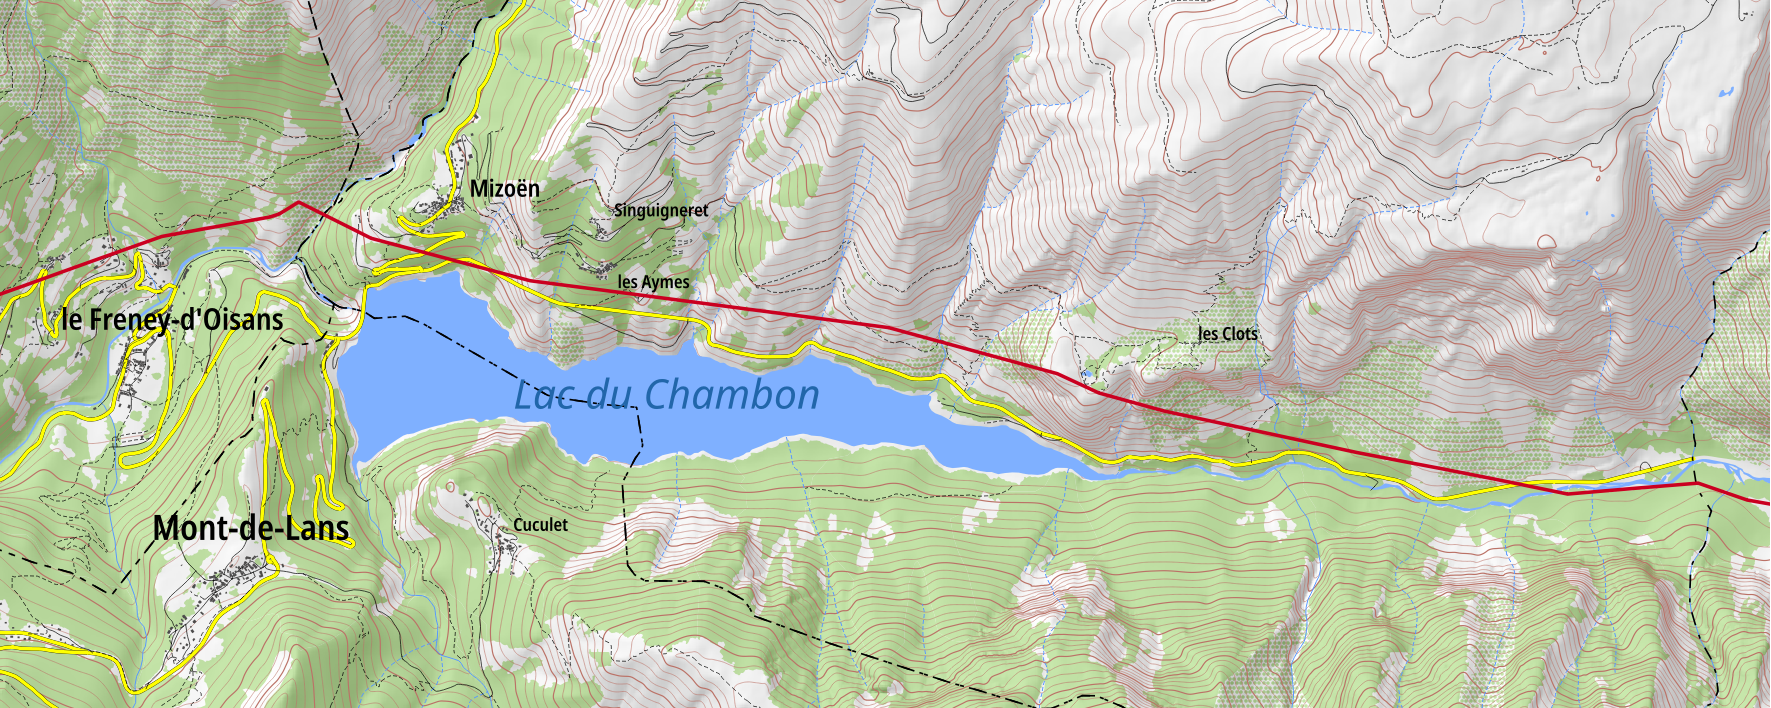
\includegraphics{./figures/Raster_vide.png}};
  %
  \begin{scope}
    \node (P2) at ([yshift=-.5cm]image.south east) {};
    \node (P1) at ([yshift=-.5cm]image.south west) {};
    % Échelle
    \node (rect) [anchor=north west, minimum width=1cm,minimum
    height=.25cm] at ([yshift=-.25cm]P1) {}; \path[draw=RdBu-9-1, line
    width=.4mm](rect.west) --([xshift=-1ex]rect.south) -- ([xshift=1ex]rect.north)
    -- (rect.east);
    \node[anchor=west, font=\tiny\vphantom{Ag}, text width = 4cm] at
    ([xshift=1ex]rect.east) {Ligne électrique utilisée comme \emph{objet de référence}};
    
    \draw[-] (P2 |- -1cm,-1cm) --++ (-1,0) node[et,pos=.5] {\SI{500}{\meter}};
    % Légende détaillée
    \path (P1) -- (P2) node[pos=.5, yshift=-1cm] {\tiny Pour la légende détaillée du fond topographique voir \autoref{anx:topo_leg}. Sources: BD TOPO 2018, BD ALTI 2018.}; 
  \end{scope}
\end{tikzpicture}
  \caption{Zone utilisée pour la comparaison des implémentations.}
  \label{fig:ZIR_HT}
\end{figure}

% Décomposition de l'indice
La \emph{relation de localisation} que nous avons identifiée comme la
plus adaptée à la formalisation de cet \emph{indice de localisation}
est \onto[orl]{Sous\-Pro\-che\-De}, traduisant une relation sur l'axe
vertical (l'altitude du \emph{sujet} est plus basse que celle de
\emph{l'objet de référence}), contrainte par une distance
planimétrique (\autoref{anx:orl_dic}). Cette \emph{relation} se
décompose en deux \emph{relations de localisation atomiques} :
\onto[orla]{Al\-ti\-tu\-de\-Stric\-te\-ment\-Inf\-érieu\-re} et
\onto[orla]{Dis\-tan\-ce\-Quan\-ti\-ta\-ti\-ve\-Pla\-ni\-mé\-tri\-que},
traduisant respectivement, la notion de position sur l'axe vertical et
la contrainte posée sur la distance planimétrique. Conformément au
\emph{principe de décomposition} et à notre méthodologie (Chapitres
\ref{chap:02} et \ref{chap:04}), la \emph{zone de localisation
  compatible} correspondant à la \emph{relation de localisation}
\onto[orl]{Sous\-Pro\-che\-De} peut être créée en intersectant les
deux \emph{zones de localisation compatibles} résultant de la
\emph{spatialisation} de ces deux \emph{relations de localisation
  atomiques.}

% Définition fonctions appartenance
La construction des \emph{zones de localisation compatibles}
correspondant à chacune des \emph{relations de localisation atomiques}
nécessite de définir des \emph{fonctions d'appartenance} ($f_A$), qui,
associent à chaque élément de l'ensemble traité, un degré ---~compris
entre 0 et 1~--- définissant l'appartenance de l'élément au
\emph{sous-ensemble flou} (Section \ref{subsec:theorie_flou}). Dans
notre contexte, où les \emph{sous-ensembles fous} représentent des
\emph{objets géographiques} et chaque élément une position, ces
fonctions définissent l'appartenance de chacune d'entre elles à la
\emph{zone de localisation compatible} construite. La définition des
\emph{fonctions d'appartenance} est donc une étape extrêmement
importante, puisqu'elle définit les règles de construction des
\emph{zones de localisation} et donc la sémantique des \emph{relations
  de localisation atomiques.} Leur définition se fait en deux étapes,
tout d'abord il faut identifier une \emph{métrique,} c'est-à-dire une
valeur quantitative ou qualitative, calculable en chaque position de
la \emph{zone initiale de recherche} et qui peut servir de mesure à la
sémantique de la \emph{relation de localisation atomique} (\eg une
distance, un angle). Puis on définit la \emph{fonction
  d'appartenance,} transformant les valeurs de la \emph{métrique} en
un \emph{degré d'appartenance.} Dans notre exemple, les
\emph{métriques} à utiliser sont assez instinctives et simples à
calculer. Par exemple, la \emph{relation de localisation atomique}
\onto[orla]{Dis\-tan\-ce\-Quan\-ti\-ta\-ti\-ve\-Pla\-ni\-mé\-tri\-que}
traduit le fait que la distance planimétrique entre le \emph{sujet} et
\emph{l'objet de référence} est faible. La métrique adaptée est donc
la distance euclidienne entre chaque position et le point le plus
proche de \emph{l'objet de référence} (\autoref{fig:ISO_DIST_HT}).

\begin{figure}
  \centering
  \begin{tikzpicture}
  \tikzset{et/.style={above,font=\footnotesize\vphantom{Ag}}}
  % 
  \node[inner sep=0pt, anchor=south west] (image) at (0,0){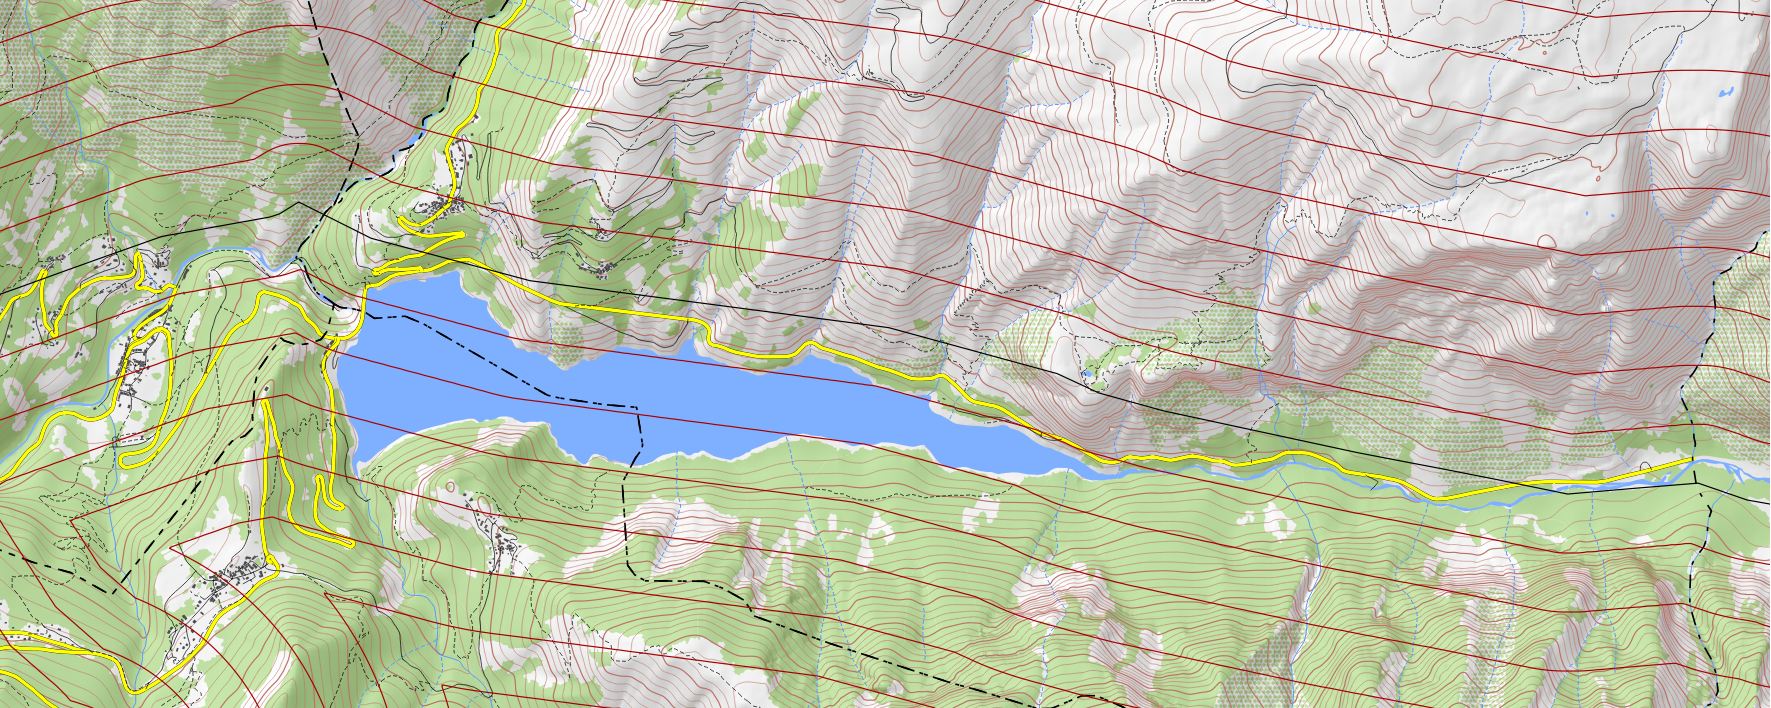
\includegraphics{./figures/Raster_ISO_DIST_HT.png}};
  % 
  \begin{scope}
    \node (P2) at ([yshift=-.5cm]image.south east) {};
    \node (P1) at ([yshift=-.5cm]image.south west) {};

    \node (rect) [anchor=north west, minimum width=1cm,minimum
    height=.25cm] at ([yshift=-.25cm]P1) {}; \path[draw=RdBu-9-1, line
    width=.4mm](rect.west) --([xshift=-1ex]rect.south) -- ([xshift=1ex]rect.north)
    -- (rect.east);
    \node[anchor=west, font=\tiny\vphantom{Ag}, text width = 4cm] at
    ([xshift=1ex]rect.east) {Ligne électrique utilisée comme
      \emph{objet de référence}};

    \node (rect2) [anchor=north west, minimum width=1cm,minimum
    height=.25cm] at ([xshift=5.5cm,yshift=-.25cm]P1) {};
    \path[draw=RdBu-9-9, line width=.25mm](rect2.west)
    --([xshift=-1ex]rect2.north) -- ([xshift=1ex]rect2.south) --
    (rect2.east); \node[anchor=west, font=\tiny\vphantom{Ag}, text
    width = 4cm] at ([xshift=1ex]rect2.east) {Isolignes d'éloignement
      à \emph{l'objet de référence} (équidistance \SI{250}{\meter})};

    % Échelle
    \draw[-] (P2 |- -1cm,-1cm) --++ (-1,0) node[et,pos=.5] {\SI{500}{\meter}};
    % Légende détaillée
    \path (P1) -- (P2) node[pos=.5, yshift=-1cm] {\tiny Pour la légende détaillée du fond topographique voir \autoref{anx:topo_leg}. Sources: BD TOPO 2018, BD ALTI 2018.}; 
  \end{scope}
\end{tikzpicture}
  \caption{\emph{Métrique} pour la \emph{relation de localisation
      atomique}    \protect\onto[orla]{Dis\-tan\-ce\-Quan\-ti\-ta\-ti\-ve\-Pla\-ni\-mé\-tri\-que}
    : La distance planaire à la ligne électrique trois brins.}
  \label{fig:ISO_DIST_HT}
\end{figure}

La \emph{relation de localisation atomique}
\onto[orla]{Al\-ti\-tu\-de\-Stric\-te\-ment\-Inf\-érieu\-re} traduit,
quant à elle, un positionnement relatif sur l'axe vertical. La
\emph{métrique} la plus adaptée est donc la différence entre
l'altitude du point le plus proche de \emph{l'objet de référence} et
l'altitude de chaque position (\autoref{fig:ISO_DALT_HT}).

\begin{figure}
  \centering
  \begin{tikzpicture}
  \tikzset{et/.style={above,font=\footnotesize\vphantom{Ag}}}
  % 
  \node[inner sep=0pt, anchor=south west] (image) at (0,0){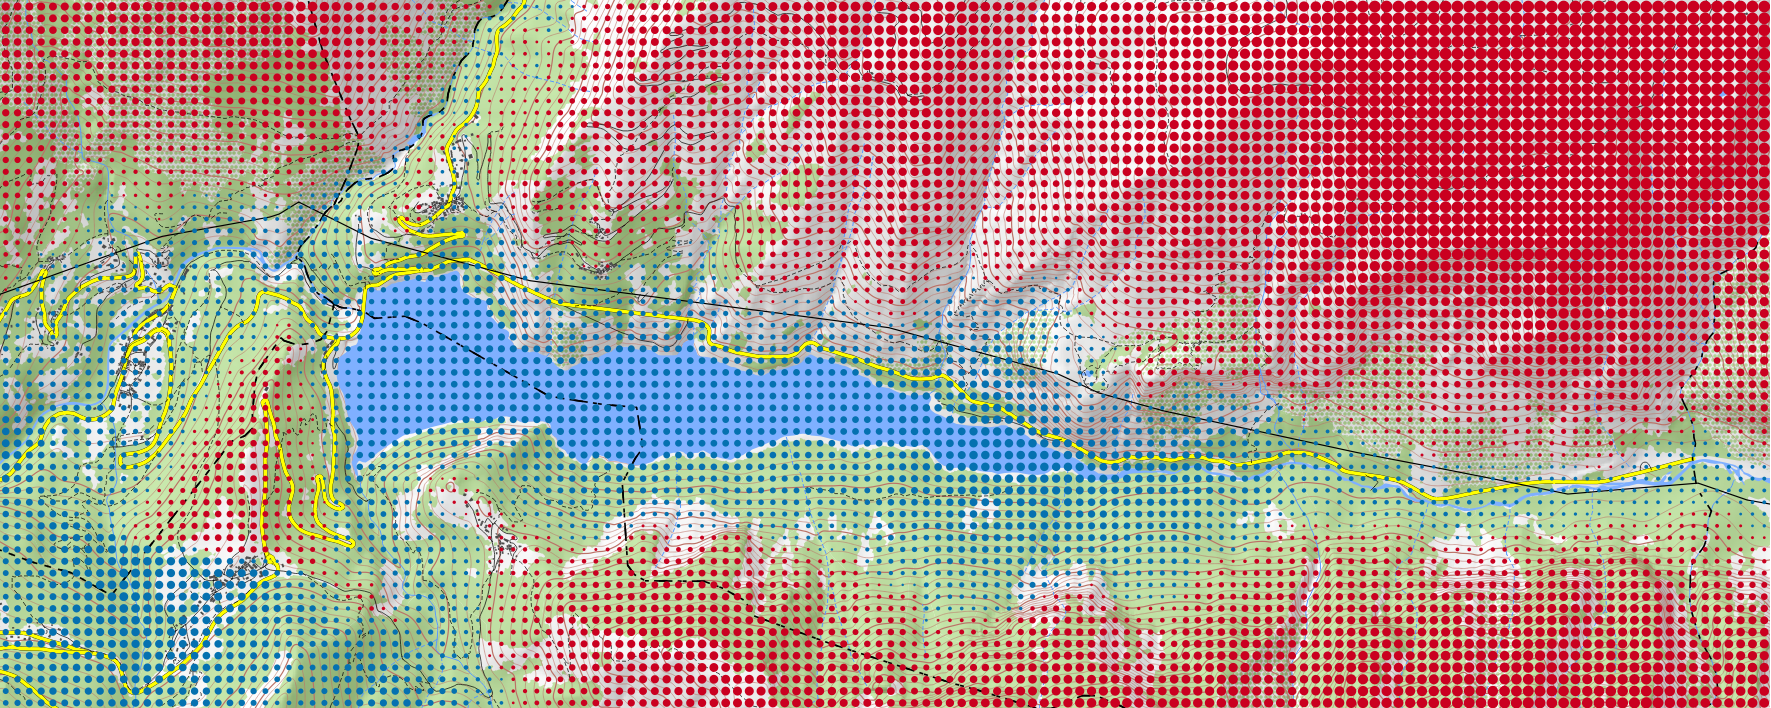
\includegraphics{./figures/Raster_ISO_DALT_HT.png}};
  % 
  \begin{scope}
    \node (P2) at ([yshift=-.5cm]image.south east) {};
    \node (P1) at ([yshift=-.5cm]image.south west) {};

    \node (rect) [anchor=north west, minimum width=1cm,minimum
    height=.25cm] at ([yshift=-.25cm]P1) {}; \path[draw=RdBu-9-1, line
    width=.4mm](rect.west) --([xshift=-1ex]rect.south) -- ([xshift=1ex]rect.north)
    -- (rect.east);
    \node[anchor=west, font=\tiny\vphantom{Ag}, text width = 4cm] at
    ([xshift=1ex]rect.east) {Ligne électrique utilisée comme
      \emph{objet de référence}};
    %
    \node[anchor=west, font=\footnotesize\vphantom{Ag}, text width=8cm] at
    (P1 |- 0cm,-1.85cm) {Différence d'altitude avec la ligne électrique};
    %
    \begin{scope}
      \foreach \x [evaluate=\xshift using 2.5+\x/10, evaluate=\rad using (\x * -.0008) + .05] in {0,...,50}
      {
        \draw[fill=RdBu-9-9,draw=none, below] ([xshift=\xshift cm, yshift=-2.5cm]P1) circle [radius=\rad cm];
      }
      \foreach \x [evaluate=\xshift using 7.5+\x/10, evaluate=\rad using (\x * .0008) + .01] in {0,...,50}
      {
        \draw[fill=RdBu-9-1,draw=none, below] ([xshift=\xshift cm, yshift=-2.5cm]P1) circle [radius=\rad cm];
      }
      % 
      \path(2.5,-3) --++ (10,0)
      node[et,pos=0] {$<$ \SI{-500}{\meter}}
      node[et,pos=.5] {\SI{0}{\meter}}
      node[et,pos=1] {$>$ \SI{500}{\meter}};
    \end{scope}
    
    % \node (rect2) [anchor=north west, minimum width=1cm,minimum
    % height=.25cm] at ([xshift=5.5cm,yshift=-.25cm]P1) {};
    % \path[draw=RdBu-9-9, line width=.25mm](rect2.west)
    % --([xshift=-1ex]rect2.north) -- ([xshift=1ex]rect2.south) --
    % (rect2.east); \node[anchor=west, font=\tiny\vphantom{Ag}, text
    % width = 4cm] at ([xshift=1ex]rect2.east) {Isolignes d'éloignement
    % à \emph{l'objet de référence} (équidistance \SI{250}{\meter})};

    % Échelle
    \draw[-] (P2 |- -1cm,-1cm) --++ (-1,0) node[et,pos=.5] {\SI{500}{\meter}};
    % Légende détaillée
    \path (P1) -- (P2) node[pos=.5, yshift=-3cm] {\tiny Pour la
      légende détaillée du fond topographique voir
      \autoref{anx:topo_leg}. Sources: BD TOPO 2018, BD ALTI 2018.};
  \end{scope}
\end{tikzpicture}
  \caption{Différence entre l'altitude locale et l'altitude de la
    ligne électrique la plus proche.}
  \label{fig:ISO_DALT_HT}
\end{figure}

La transformation des valeurs de ces deux métriques en degré
d'appartenance se fait à l'aide d'une fonction d'appartenance qu'il
convient de définir. Pour ce faire nous procédons généralement en deux
étapes. La première consiste à identifier la forme de \emph{la
  fonction d'appartenance} qui nous semble être la plus pertinente
pour retranscrire la sémantique de la \emph{relation de localisation
  atomique.} Puis nous identifions les seuils de cette
fonction. Ainsi, la première étape permet \footnote{Conjointement à la
  sélection d'une \emph{métrique.}} de fixer la sémantique de la
\emph{relation,} alors que la seconde étape fait plus office de
paramétrisation fine. La sélection de la forme de la fonction ne pose
pas de problèmes particuliers, contrairement à la définition des
seuils qui, comme nous allons le voir, est généralement assez
arbitraire. Cependant, pour cet exemple particulier les seuils définis
ont été validés par un secouriste du \ac{pghm}.

La \emph{relation de localisation atomique}
\onto[orla]{Dis\-tan\-ce\-Quan\-ti\-ta\-ti\-ve\-Pla\-ni\-mé\-tri\-que}
est utilisée pour figurer le fait que le \emph{sujet} n'est pas très
éloigné de \emph{l'objet de référence.} Ainsi, une position
\enquote{proche} de \emph{l'objet de référence} doit avoir un
\emph{degré d'appartenance} à la \emph{zone de localisation
  compatible} correspondant à cette \emph{relation de localisation
  atomique} plus élevé qu'une position qui en est éloigné. Le degré
d'appartenance doit donc diminuer lorsque la distance à \emph{l'objet
  de référence} (\ie la valeur de la métrique) augmente. La forme de
la fonction d'appartenance étant fixée, nous pouvons à présent en
définir les seuils. Deux valeurs sont à fixer, la première est la
distance à partir de laquelle le degré d'appartenance décroit. Si elle
est nulle le degré d’appartenance décroit dès que la distance
augmente, sinon il y aura une zone, dont la largeur dépend de la
valeur choisie, où le degré d'appartenance sera maximal. Définir ce
premier seuil revient à se demander quelle est la distance à partir de
laquelle on ne peut plus considérer que l'on est \enquote{proche}
d'une ligne électrique. Pour cet exemple nous avons fixé empiriquement
cette valeur à \SI{50}{\meter}. Le second seuil à fixer est la
distance à partir de laquelle le degré d'appartenance est nul. De
manière tout aussi empirique, nous avons fixé cette valeur à
\SI{100}{\meter}. Ainsi, entre 0 et 50 mètres, le degré d'appartenance
est de 1, puis il décroit jusqu’à être de 0 à 100 mètres et reste nul
au-delà, comme le montre la figure \ref{fig:fnc_app_Dist}.

La définition de la forme de la fonction d'appartenance pour la
\emph{relation de localisation atomique}
\onto[orla]{Al\-ti\-tu\-de\-Stric\-te\-ment\-Inf\-érieu\-re} ne pose
pas non plus de problèmes particuliers. Comme cette \emph{relation}
traduit une position relative sur l'axe vertical, le degré
d'appartenance doit être à 1 lorsque l'altitude de la position est
inférieure à celle de \emph{l'objet de référence} (\ie que la métrique
est négative) et nul dans le cas contraire (\ie que la métrique est
positive). Il faut alors définir les valeurs de la métrique à partir
desquelles le degré d'appartenance est de 1 ou de 0. Étant donné que
la différence d'altitude est calculée à partir du sommet de la ligne
électrique nous avons considéré que toute position dont l'altitude
était inférieure au point le plus proche de la ligne électrique (\ie
dès que la valeur de la métrique est négative) avait un degré
d'appartenance de 1. Nous avons fixé le second seuil à \SI{5}{\meter},
ce qui permet d'ajouter une petite marge d'erreur. Ainsi, le degré
d'appartenance est de 1 jusqu’à ce que la différence d'altitude soit
nulle, puis il décroit rapidement jusqu'à atteindre la valeur de 0
lorsque la différence est de \SI{5}{\meter} (\ie que la position est
\SI{5}{\meter} au-dessus du sommet de la ligne électrique), la valeur
reste nulle au-delà (Figure \ref{fig:fnc_app_AltInf}).

\begin{figure}
  \centering \subfloat[]{%
    \begin{tikzpicture}[scale=.7]
  \def\decalageX{-.2}
  \def\decalageY{-.2}
  % Courbe
  \begin{scope}[transparency group]
    % fond
    \begin{scope}
      \path[ffa] (0,2) -- (2.5,2) -- (5, 0)  -- (0,0) -- cycle;
    \end{scope}
    % bords
    \begin{scope}
      \path[ffc] (0,2) -- (2.5,2) -- (5, 0) -++ (3,0) ;
      \path[ffc_fade] (8,0) -- (9,0) ;
    \end{scope}
  \end{scope}
  % Axes X, Y
  \begin{scope}
    % Axe X
    \begin{scope}
      % Axe
      \draw[->] (0, \decalageX) --++ (9, 0) coordinate (x axis);
      % Graduations
      \foreach \n/\t in {0/{0},1/{20},2/{40},3/{60},4/{80},5/{100},6/{120},7/{140},8/{160}}
      {
        \draw[-] (\n, \decalageX - .05) --++ (0, .1);
        \node[below, font=\footnotesize] at (\n, \decalageX - .05) {\t};
      }
      % label
      \node[above left, yshift=.1cm, font=\small] at (x axis) {$Distance\ (m)$};
    \end{scope}
    % Axe Y
    \begin{scope}
      % Axe
      \draw[-] (\decalageY ,0) --++ (0, 2) coordinate (y axis);
      % Graduations
      \foreach \n/\t in {0/{0},2/{1}}
      {
        \draw[-] (\decalageY -.05, \n) --++ (.1, 0);
        \node[left, font=\footnotesize] at (\decalageY -.05, \n) {\t};
      }
      % Label
      \node[above] at (y axis) {$\mu$};
    \end{scope}
  \end{scope}
  \begin{scope}
    % Seuil 1
    \draw[ffc,line width=.5] (2.5,\decalageY) -- (2.5,2);
    \draw[fill, RdBu-9-1] (2.5,\decalageY) circle (2pt);
    \draw[fill, RdBu-9-1] (2.5,2) circle (2pt);
    % Seuil 2
    \draw[ffc,line width=.5] (5,\decalageY) -- (5,0);
    \draw[fill, RdBu-9-1] (5,\decalageY) circle (2pt);
    \draw[fill, RdBu-9-1] (5,0) circle (2pt);
  \end{scope}
\end{tikzpicture}

    \label{fig:fnc_app_Dist}
  }
  \hfill%
  \subfloat[]{%
    \begin{tikzpicture}[scale=.75]
  \def\decalageX{-.2}
  \def\decalageY{-.2}
  % Courbe
  \begin{scope}[transparency group]
    % fond
    \begin{scope}
      \draw[ffa] (1,2) -- (4.5, 2) -- (5.5,0) -- (1,0)-- cycle;
      \draw[ffa_fade_m] (0,2) -- (1, 2) -- (1,0) -- (0,0)-- cycle;
    \end{scope}
    % bords
    \begin{scope}
      \path[ffc] (1, 2) --(4.5, 2) -- (5.5,0) -- (8,0);
      \path[ffc_fade_m] (0,2) -- (1,2);
      \path[ffc_fade] (8,0) -- (9,0) ;
    \end{scope}
  \end{scope}
  % Axes
  \begin{scope}
    % Axe X
    \begin{scope}
      % Axe
      \draw[<->] (0, \decalageX) --++ (9, 0) coordinate (x axis);
      % Graduations
      \foreach \n/\t in {.5/{-20},1.5/{-15},2.5/{-10},3.5/{-5},4.5/{0},5.5/{5},6.5/{10},7.5/{15},8.5/{20}}
      {
        \draw[-] (\n, \decalageX - .05) --++ (0, .1);
        \node[below, font=\footnotesize] at (\n, \decalageX - .05) {\t};
      }
      % label
      \node[above left, yshift=.1cm, font=\small] at (x axis) {$\Delta\,Altitude\,(m)$};
    \end{scope}
    % Axe Y
    \begin{scope}
      % Axe
      \draw[-] (\decalageY ,0) --++ (0, 2) coordinate (y axis);
      % Graduations
      \foreach \n/\t in {0/{0},2/{1}}
      {
        \draw[-] (\decalageY -.05, \n) --++ (.1, 0);
        \node[left, font=\footnotesize] at (\decalageY -.05, \n) {\t};
      }
      % Label
      \node[above] at (y axis) {$\mu$};
    \end{scope}
  \end{scope}
  % Analyse
  \begin{scope}
    \draw (4.5,0) -- (4.5,2);
    \draw[fill] (4.5,0) circle (1pt);
    \draw[fill] (4.5,2) circle (1pt);
    \node[above] at (4.5,2) {P};
  \end{scope}
\end{tikzpicture}

    \label{fig:fnc_app_AltInf}
  }
  \caption{Fonctions d'appartenance pour les \emph{relations de
      localisation atomiques}
    \protect\onto[orla]{Dis\-tan\-ce\-Quan\-ti\-ta\-ti\-ve\-Pla\-ni\-mé\-tri\-que}
    \protect\subref{fig:fnc_app_Dist} et
    \protect\onto[orla]{Al\-ti\-tu\-de\-Stric\-te\-ment\-Inf\-érieu\-re}
    \protect\subref{fig:fnc_app_AltInf}, utilisées pour construire la
    \emph{zone de localisation probable} de \emph{l'indice de
      localisation} \enquote{je suis sous une ligne électrique trois
      brins}.}
  \label{fig:fnc_app_sousProche}
\end{figure}

La construction de la \emph{zone de localisation probable} nécessite
de \emph{fusionner} ---~à l'aide d'une intersection~--- les deux
\emph{zones de localisations compatibles} correspondant aux
\emph{relations de localisation atomiques}
\onto[orla]{Al\-ti\-tu\-de\-Stric\-te\-ment\-Inf\-érieu\-re} et
\onto[orla]{Dis\-tan\-ce\-Quan\-ti\-ta\-ti\-ve\-Pla\-ni\-mé\-tri\-que}. Si
son appliquation est dépendante de l'implémentation, la méthode
utilisée est fixée par le modèle théorique. La \emph{théorie des
  sous-ensembles flous} nécessite d'employer une \emph{t-norme.} Étant
donné que cette comparaison ne porte que sur les implémenations et non
sur les opérateurs d'unions et d'intersection, nous avons choisi
d'utiliser les opérateurs les plus courants, ceux proposés par
\textcite{Zadeh1965}, où la fonction \emph{minimum} fait office de
\emph{t-norme.}

\subsection{Implémentation raster}

L'implémentation a l'avantage d'être extrêmement facile a mettre en
place. Une fois que les \emph{métriques} et les \emph{fonctions
  d’appartenance} ont été définies, elle se résume à calculer, pour
chaque pixel d'une grille échantillonnant l'espace, la valeur de la
\emph{métrique,} puis du degré d'appartenance à la \emph{zone de
  localisation compatible} \emph{spatialisée.} Cette opération est
répétée pour chaque \emph{relation de localisation atomique,} puis les
\emph{zones de localisation compatibles} résultantes sont
\emph{fusionnées} à l'aide des opérateurs d'intersection et de fusion
sélectionnés. Le seul choix imposé par l'utilisation de cette
implémentation et celui de la résolution du raster. Ce critère fixe la
taille et le nombre de pixels du raster et influe, par conséquent, sur
la précision et la durée du calcul. Cette résolution doit être
suffisamment grande pour permettre le calcul des fonctions
\emph{d'appartenance définies.} Par exemple, la \emph{fonction
  d'appartenance} définie pour la \emph{relation de localisation
  atomique}
\onto[orla]{Dis\-tan\-ce\-Quan\-ti\-ta\-ti\-ve\-Pla\-ni\-mé\-tri\-que}
(figure \ref{fig:fnc_app_Dist}) a deux seuils, \num{50} et
\SI{100}{\meter}.

L’application de la fonction d'appartenance (figure
\ref{fig:fnc_app_Dist}) à la métrique précédemment calculée (figure
\ref{fig:ISO_DIST_HT}) permet d'obtenir la figure
\ref{fig:ZLC_DIST_HT}, représentant la \emph{zone de localisation
  compatible} de la \emph{relation de localisation atomique}
\onto[orla]{Dis\-tan\-ce\-Quan\-ti\-ta\-ti\-ve\-Pla\-ni\-mé\-tri\-que}.
Le degré d'appartenance de chaque pixel à la \emph{zone de
  localisation compatible} est représenté par un cercle, centré sur le
pixel et dont le diamètre augmente avec celui-ci. Lorsque ce degré est
maximal, le diamètre du cercle est égal à la maille du raster (50
mètres dans le cas présent). Le diamètre est minimal lorsque le degré
d'appartenance est supérieur à zéro et les valeurs nulles sont
filtrées pour faciliter la lisibilité.

\begin{figure}
  \centering
  \begin{tikzpicture}
  \tikzset{et/.style={above,font=\footnotesize\vphantom{Ag}}}
  % 
  \node[inner sep=0pt, anchor=south west] (image) at (0,0){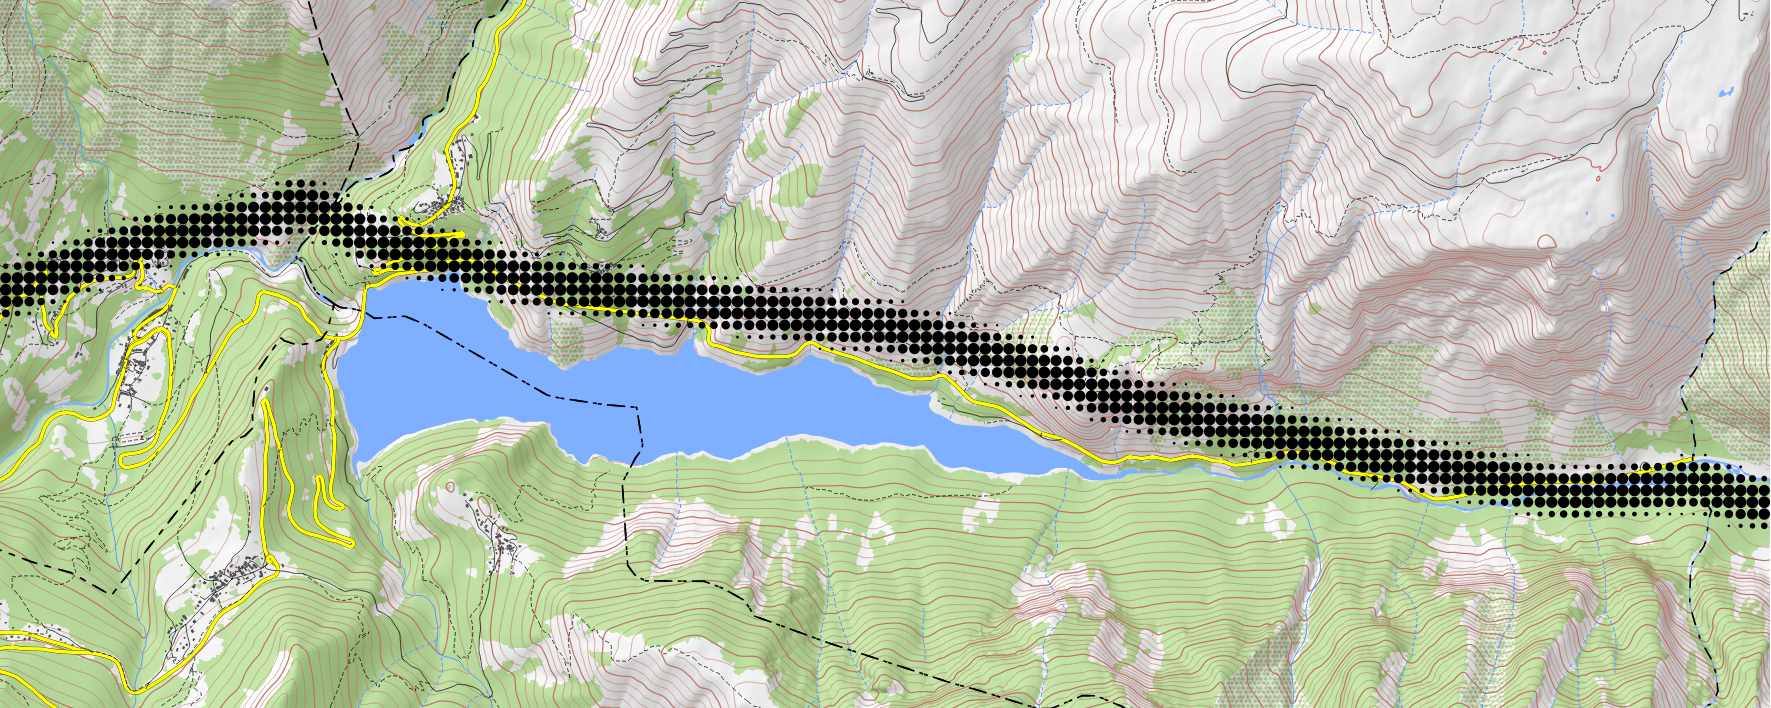
\includegraphics{./figures/Raster_ZLC_DIST_HT.png}};
  % 
  \begin{scope}
    \node (P2) at ([yshift=-.5cm]image.south east) {};
    \node (P1) at ([yshift=-.5cm]image.south west) {};
    % 
    \node (rect) [anchor=north west, minimum width=1cm,minimum
    height=.25cm] at ([yshift=-.25cm]P1) {}; \path[draw=RdBu-9-1, line
    width=.4mm](rect.west) --([xshift=-1ex]rect.south) -- ([xshift=1ex]rect.north)
    -- (rect.east);
    \node[anchor=west, font=\tiny\vphantom{Ag}, text width = 4cm] at
    ([xshift=1ex]rect.east) {Ligne électrique utilisée comme
      \emph{objet de référence}};

    \foreach \x [evaluate=\xshift using \x/10, evaluate=\rad using (\x * .0004) + .01] in {0,...,100}
    {
      \draw[fill=black,draw=none, below] ([xshift=\xshift cm, yshift=-1.5cm]P1) circle [radius=\rad cm];
    }
    % 
    \path(P1 |- 0cm,-2cm) --++ (10,0)
    node[et,pos=0] {0}
    node[et,pos=.1] {0,1}
    node[et,pos=.2] {0,2}
    node[et,pos=.3] {0,3}
    node[et,pos=.4] {0,4}
    node[et,pos=.65] {0,65}
    node[et,pos=1] {1};
    % Échelle
    \draw[-] (P2 |- -1cm,-1cm) --++ (-1,0) node[et,pos=.5] {\SI{500}{\meter}};
    % Légende détaillée
    \path (P1) -- (P2) node[pos=.5, yshift=-2cm] {\tiny Pour la légende détaillée du fond topographique voir \autoref{anx:topo_leg}. Sources: BD TOPO 2018, BD ALTI 2018.}; 
  \end{scope}
\end{tikzpicture}
  \caption{\emph{Zone de localisation compatible} pour la
    \emph{relation de localisation atomique}
    \protect\onto[orla]{Dis\-tan\-ce\-Quan\-ti\-ta\-ti\-ve\-Pla\-ni\-mé\-tri\-que}.}
  \label{fig:ZLC_DIST_HT}
\end{figure}

Une méthode identique est utilisée pour construire la \emph{zone de
  localisation compatible} issue de la \emph{spatialisation} de la
\emph{relation de localisation atomique}
\onto[orla]{Al\-ti\-tu\-de\-Stric\-te\-ment\-Inf\-érieu\-re}. La
\emph{métrique} identifiée (figure \ref{fig:ISO_DALT_HT}) est calculé
pour chaque pixel, puis ces valeurs sont transformées en \emph{degrés
  d'appartenance} à l'aide de fonction d'appartenance définie
précédemment (Figure \ref{fig:fnc_app_AltInf}). La figure
\ref{fig:ZLC_ALTINF_HT}, qui résulte de ce processus, représente alors
le degré d'appartenance de chaque pixel à la \emph{zone de
  localisation compatible.}

\begin{figure}
  \centering
  \begin{tikzpicture}
  \tikzset{et/.style={above,font=\footnotesize\vphantom{Ag}}}
  %
  \node[inner sep=0pt, anchor=south west] (image) at (0,0){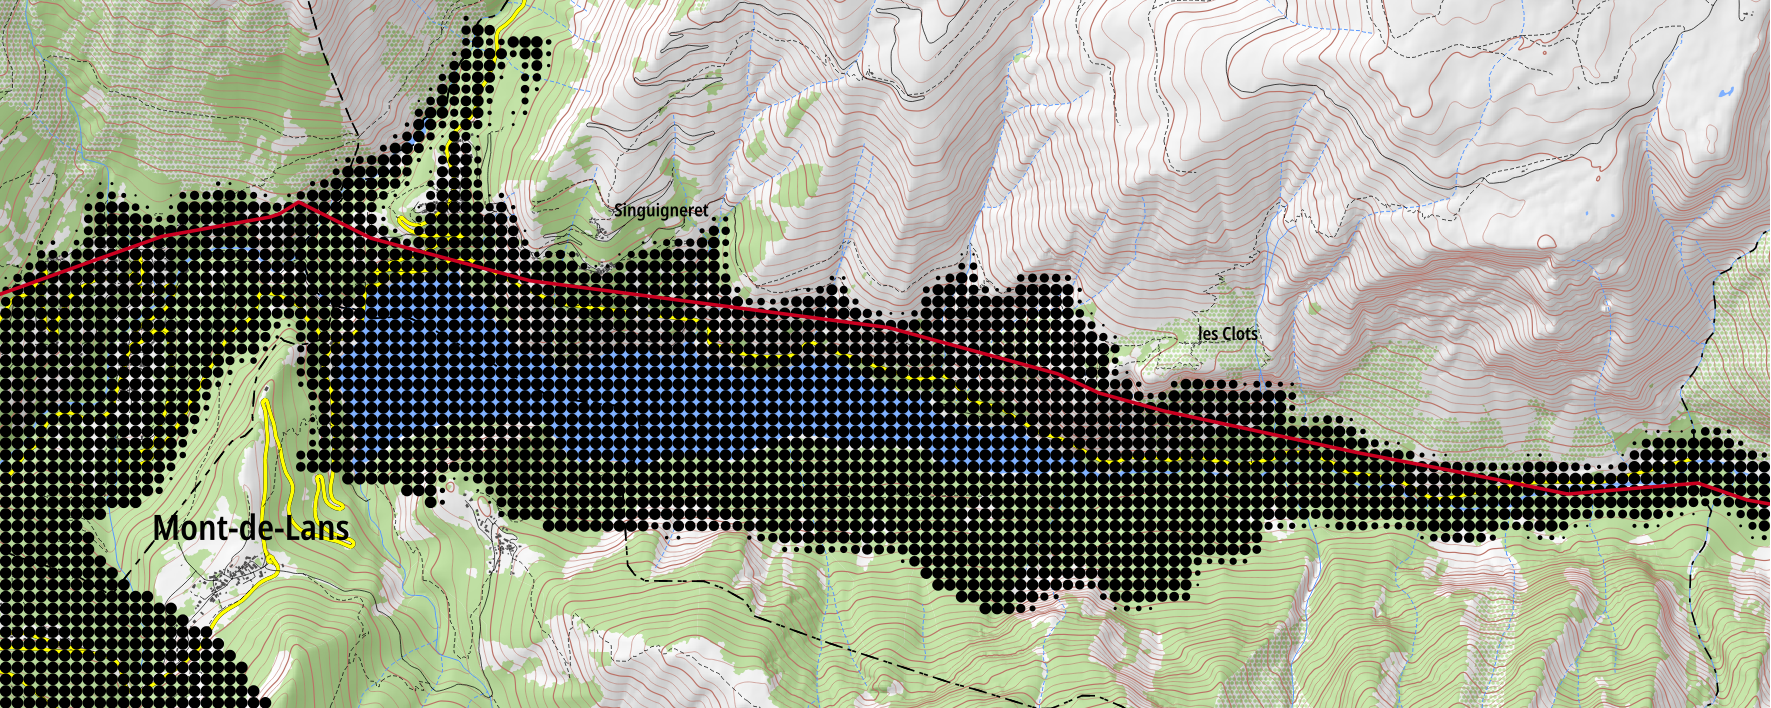
\includegraphics{./figures/Raster_ZLC_ALTINF_HT.png}};
  %
  \begin{scope}
    \node (P2) at ([yshift=-.5cm]image.south east) {};
    \node (P1) at ([yshift=-.5cm]image.south west) {};
    %
    \node (rect) [anchor=north west, minimum width=1cm,minimum
    height=.25cm] at ([yshift=-.25cm]P1) {}; \path[draw=RdBu-9-1, line
    width=.4mm](rect.west) --([xshift=-1ex]rect.south) -- ([xshift=1ex]rect.north)
    -- (rect.east);
    \node[anchor=west, font=\tiny\vphantom{Ag}, text width = 4cm] at
    ([xshift=1ex]rect.east) {Ligne électrique utilisée comme
      \emph{objet de référence}};

    \foreach \x [evaluate=\xshift using \x/10, evaluate=\rad using (\x * .0004) + .01] in {0,...,100}
    {
      \draw[fill=black,draw=none, below] ([xshift=\xshift cm, yshift=-1.5cm]P1) circle [radius=\rad cm];
    }
    % 
    \path(P1 |- 0cm,-2cm) --++ (10,0)
    node[et,pos=0] {0}
    node[et,pos=.1] {0,1}
    node[et,pos=.2] {0,2}
    node[et,pos=.3] {0,3}
    node[et,pos=.4] {0,4}
    node[et,pos=.65] {0,65}
    node[et,pos=1] {1};
    % Échelle
    \draw[-] (P2 |- -1cm,-1cm) --++ (-1,0) node[et,pos=.5] {\SI{500}{\meter}};
    % Légende détaillée
    \path (P1) -- (P2) node[pos=.5, yshift=-2cm] {\tiny Pour la légende détaillée du fond topographique voir \autoref{anx:topo_leg}. Sources: BD TOPO 2018, BD ALTI 2018.}; 
  \end{scope}
\end{tikzpicture}
  \caption{\emph{Zone de localisation compatible} pour la
    \emph{relation de localisation atomique}
    \protect\onto[orla]{Al\-ti\-tu\-de\-Stric\-te\-ment\-Inf\-érieu\-re}.}
  \label{fig:ZLC_ALTINF_HT}
\end{figure}

Les rasters représentant les deux \emph{zones de localisation
  compatibles} à intersecter possédant les mêmes résolutions et
étendues, il y a bijection entre deux ensembles de pixels. On peut
alors, sans effectuer de ré-échantillonnage, appliquer un opérateur
d'intersection à chaque paire de pixels représentant la même
position. Après l'intersection des \emph{zones de localisation
  compatibles} figurées sur les figures \ref{fig:ZLC_DIST_HT} et
\ref{fig:ZLC_ALTINF_HT} on obtient la \emph{zone de localisation
  probable} (figure \ref{fig:ZLP_SOUS_HT}) correspondant à l'ensemble
des positions situées \emph{à proximité} et à une \emph{altitude
  inférieure} de la ligne à haute-tension. Comme on peut le voir, le
résultat obtenu est semblable à la figure \ref{fig:ZLC_DIST_HT} et
assez différent de la figure \ref{fig:ZLC_ALTINF_HT}. L'étendue de la
\emph{zone de localisation probable} est donc plus contraint par
l'éloignement à la ligne électrique que par la différence
d'altitude. Pour le dire autrement, il y a peu de positions
\enquote{proches} et \enquote{au-dessus} d'une ligne électrique.

\begin{figure}
  \centering
  \begin{tikzpicture}
  \tikzset{et/.style={above,font=\footnotesize\vphantom{Ag}}}
  % 
  \node[inner sep=0pt, anchor=south west] (image) at (0,0){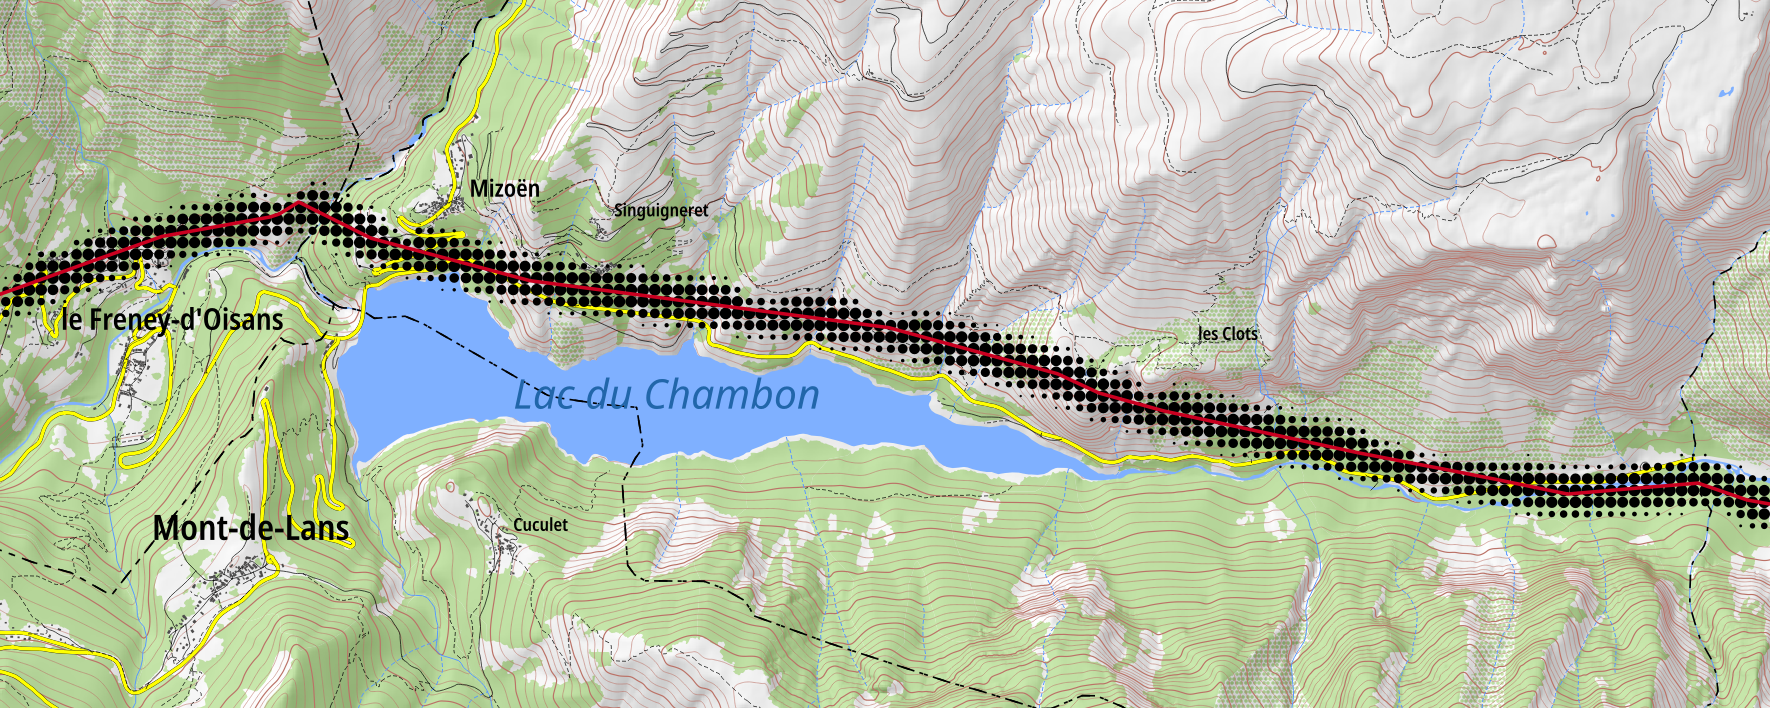
\includegraphics{./figures/Raster_ZLP_SOUS_HT.png}};
  % 
  \begin{scope}
    \node (P2) at ([yshift=-.5cm]image.south east) {};
    \node (P1) at ([yshift=-.5cm]image.south west) {};
    % 
    \node (rect) [anchor=north west, minimum width=1cm,minimum
    height=.25cm] at ([yshift=-.25cm]P1) {}; \path[draw=RdBu-9-1, line
    width=.4mm](rect.west) --([xshift=-1ex]rect.south) -- ([xshift=1ex]rect.north)
    -- (rect.east);
    \node[anchor=west, font=\tiny\vphantom{Ag}, text width = 4cm] at
    ([xshift=1ex]rect.east) {Ligne électrique utilisée comme
      \emph{objet de référence}};

    \foreach \x [evaluate=\xshift using \x/10, evaluate=\rad using (\x * .0004) + .01] in {0,...,100}
    {
      \draw[fill=black,draw=none, below] ([xshift=\xshift cm, yshift=-1.5cm]P1) circle [radius=\rad cm];
    }
    % 
    \path(P1 |- 0cm,-2cm) --++ (10,0)
    node[et,pos=0] {0}
    node[et,pos=.1] {0,1}
    node[et,pos=.2] {0,2}
    node[et,pos=.3] {0,3}
    node[et,pos=.4] {0,4}
    node[et,pos=.65] {0,65}
    node[et,pos=1] {1};
    % Échelle
    \draw[-] (P2 |- -1cm,-1cm) --++ (-1,0) node[et,pos=.5] {\SI{500}{\meter}};
    % Légende détaillée
    \path (P1) -- (P2) node[pos=.5, yshift=-2cm] {\tiny Pour la légende détaillée du fond topographique voir \autoref{anx:topo_leg}. Sources: BD TOPO 2018, BD ALTI 2018.}; 
  \end{scope}
\end{tikzpicture}
  \caption{\emph{Zone de localisation probable} pour \emph{l'indice de
      localisation} \enquote{Je suis sous une ligne électrique trois
      brins}.}
  \label{fig:ZLP_SOUS_HT}
\end{figure}


\subsection{Implémentation par \emph{Alpha-cuts}}

Bien que fondée sur les mêmes aspects théoriques que l'implémentation
raster, l'implémentation par \emph{alpha-cuts} propose une approche
très différente. On pourrait construire des \emph{alpha-cuts} de
plusieurs manières. Une première solution serait de partir des
résultats de l'implémentation raster (\autoref{fig:ZLP_SOUS_HT}) et
d'en extraire les pixels dont le degré d'appartenance est supérieur à
un seuil fixé. Cette construction par sélection \footnote{Fortement
  semblable à la \emph{construction en extension d'ordre supérieur}
  présentée dans le \autoref{chap:03}.}, n'est cependant rien de plus
qu'un post-traitement des résultats de l'implémentation raster et elle
ne possède pas d'avantages (ou inconvénients) qui lui soient
propres. Une approche différente est cependant
envisageable. \textcite{Runz2008a, Zoghlami2016}, par exemple, des
\emph{alpha-cuts} directement, sans passer par une étape préalable de
calcul des degrés d'appartenance, soit une \emph{construction en
  intension} (\autoref{:chap:03}). La construction \emph{d'alpha-cuts}
en intension demande d'identifier les critères jouant sur la forme de
la \emph{zone de localisation,} soit, dans notre exemple, la distance
et différence d'altitude par rapport à la ligne
électrique. Conformément au \emph{principe de décomposition} on peut
alors définir une méthode géométrique permettant de construire, pour
chaque \emph{relation de localisation atomique} et chaque
\emph{alpha-cut} construite, une région, correspondant à une
\emph{alpha-cut} de la \emph{zone de localisation compatible}
traitée. Ces différentes \emph{alpha-cuts} seraient alors intersectées
deux à deux, par même degré d'appartenance en vue d'obtenir les
\emph{alpha-cuts} de la \emph{zone de localisation probable} et ce de
manière fortement similaire à l'implémentation raster. Pour cette
comparaison nous avons choisi de construire trois \emph{alpha-cuts,}
celle dont le degré est égal à 1, délimitant le \emph{noyau} du
\emph{sous-ensemble flou,} celle dont le degré d'appartenance est
supérieur à 0, délimitant le \emph{support} et enfin
\emph{l'alpha-cut} de degré 0,5.

% Détail de la méthode
Pour chaque segment de la ligne électrique traitée, nous construisons
un polyèdre, correspondant à une \emph{alpha-cut}
tridimensionnelle. Aucun \ac{sig} ne permettant de construire ce type
d'objets, nous avons été contrains de nous orienter vers une solution
de plus bas niveau, la bibliothèque de calcul géométrique CGAL
\autocite{CGAL2019}, ce qui a considérablement complexifié la
tâche. Le polyèdre construit se compose de 6 faces, définies par
autant de demis-plans (\autoref{schema_polyhedre}). Comme les
\emph{alpha-cuts} délimitent une \emph{zone de localisation}
dépendante, toutes choses égales par ailleurs, de la position de
\emph{l'objet de référence,} la position de tous ces demi-plans est
exprimable en fonction de la position de la ligne électrique
traitée. Toutefois, certains d'entre eux ont une position variante par
translation, en fonction de \emph{l'alpha-cut} considérée.

Les demi-plans dont la position varie en fonction de
\emph{l'alpha-cut} considérée sont ceux dont la position délimite une
zone de même degré d'appartenance. Par exemple, les demis-plans
latéraux (\ie situés à gauche et à droite par rapport au sens de la
ligne électrique et parallèlement à celle-ci) permettent de délimiter
une distance planimétrique à \emph{l'objet de référence} et donc de
représenter la \emph{relation de localisation atomique}
\onto[orla]{Dis\-tan\-ce\-Quan\-ti\-ta\-ti\-ve\-Pla\-ni\-mé\-tri\-que}. Si
l'on cherche à construire \emph{l'alpha-cut} délimitant le support, il
faudra placer ces demi-plans latéraux de manière a ce qu'aucune
position située au-delà (par rapport à la ligne électrique) ne puisse
avoir un degré d'appartenance non nul. Dans le cas de \emph{l'indice
  de localisation} considéré, seule la \emph{relation}
\onto[orla]{Dis\-tan\-ce\-Quan\-ti\-dta\-ti\-ve\-Pla\-ni\-mé\-tri\-que}
impacte la position de ces deux demi-plans, on peut alors se fonder
sur la fonction d'appartenance correspondante (Figure
\ref{fig:fnc_app_Dist}) et identifier la distance correspondant au
degré d'éloignement considéré, soit \SI{100}{\meter} pour un degré
d'appartenance non nul. Les demi-plans avant et arrière délimitent
également la distance planimétrique à la ligne électrique. Cependant
nous avons choisi de ne pas les faire varier. D'une part, car nous
travaillons sur un seul \emph{objet de référence,} traversant l'aire
étudiée de part en part et sans changement de direction marqués. Par
conséquent, les polyèdres modélisant les \emph{alpha-cuts} de chaque
segment sont toutes en contact par leurs faces avant et arrières, la
prise en compte de leur décalage par rapport à la ligne électrique
n'est donc pas nécessaire. De plus, contrairement aux faces latérales,
les limites avant et arrières des \emph{alpha-cuts} ne peuvent être
délimitées de manière satisfaisante par des demi-plans.
% 
Comme les demi-plans latéraux, la position du demi-plan supérieur
dépend de la ligne électrique considérée et de \emph{l'alpha-cut}
traitée. Sa position varie en fonction de la \emph{relation de
  localisation atomique}
\onto[orla]{Al\-ti\-tu\-de\-Stric\-te\-ment\-Inf\-érieu\-re}. Ainsi,
si \emph{l'alpha-cut} modélisée est la limite du \emph{support,} le
demi-plan supérieur doit être placé de manière à ce que toutes les
positions situées au-delà aient un degré d'appartenance nul, il est
donc placé \SI{5}{\meter} au-dessus de la ligne électrique.  Enfin, le
demi-plan inférieur ne sert qu'a fermer le polyèdre, aucune des
\emph{relations de localisation} n'imposant une limite d'altitude
minimale. Pour éviter de réduire artificiellement l'étendue des
\emph{alpha-cuts} nous avons placé ce demi-plan a une altitude
nettement plus faible que l'altitude minimale de la \ac{zir}, simulant
ainsi un demi-plan virtuellement à l'infini. Le résultat de
l'implémentation par \emph{alpha-cuts} est visible sur les figures
\ref{fig:AlphaCuts_coupe} et \ref{fig:AlphaCuts_zenith}.

\begin{figure}
  \centering
  % \begin{tikzpicture}[x={(1cm,0cm)}, y={(0cm,1cm)}, z={(3.85mm, 3.85mm)}]
  \coordinate (Ld) at (2,4,6);
  \coordinate (Lf) at (8,2,2); 	

  \coordinate (A) at ($(Ld) - (0,4,-2)$); 
  \coordinate (B) at ($(Lf) - (0,2,-2)$); 
  \coordinate (C) at ($(Lf) - (0,2, 2)$);
  \coordinate (D) at ($(Ld) - (0,4, 2)$); 



  \begin{scope}[canvas is xz plane at y=0]
    \draw (0,0) grid (10,10);
  \end{scope}



  \begin{scope}
    \draw[fill=red] (A) -- (B) -- (C) -- (D) -- cycle;
    % \draw[fill=red] (2,0,6) --++(3,0,0) --++(0,3,0) --++(-3,-1,0) -- cycle;
    

    % \draw[fill=red] (2,0,4) --++(3,0,0) --++(0,3,0) --++(-3,-1,0) -- cycle;
  \end{scope}

  \path[draw] (Ld) -- (Lf);
    \path[draw] (Ld) --++ (0,-4,0);
  \path[draw] (Lf) --++ (0,-2,0);
  
\end{tikzpicture}
  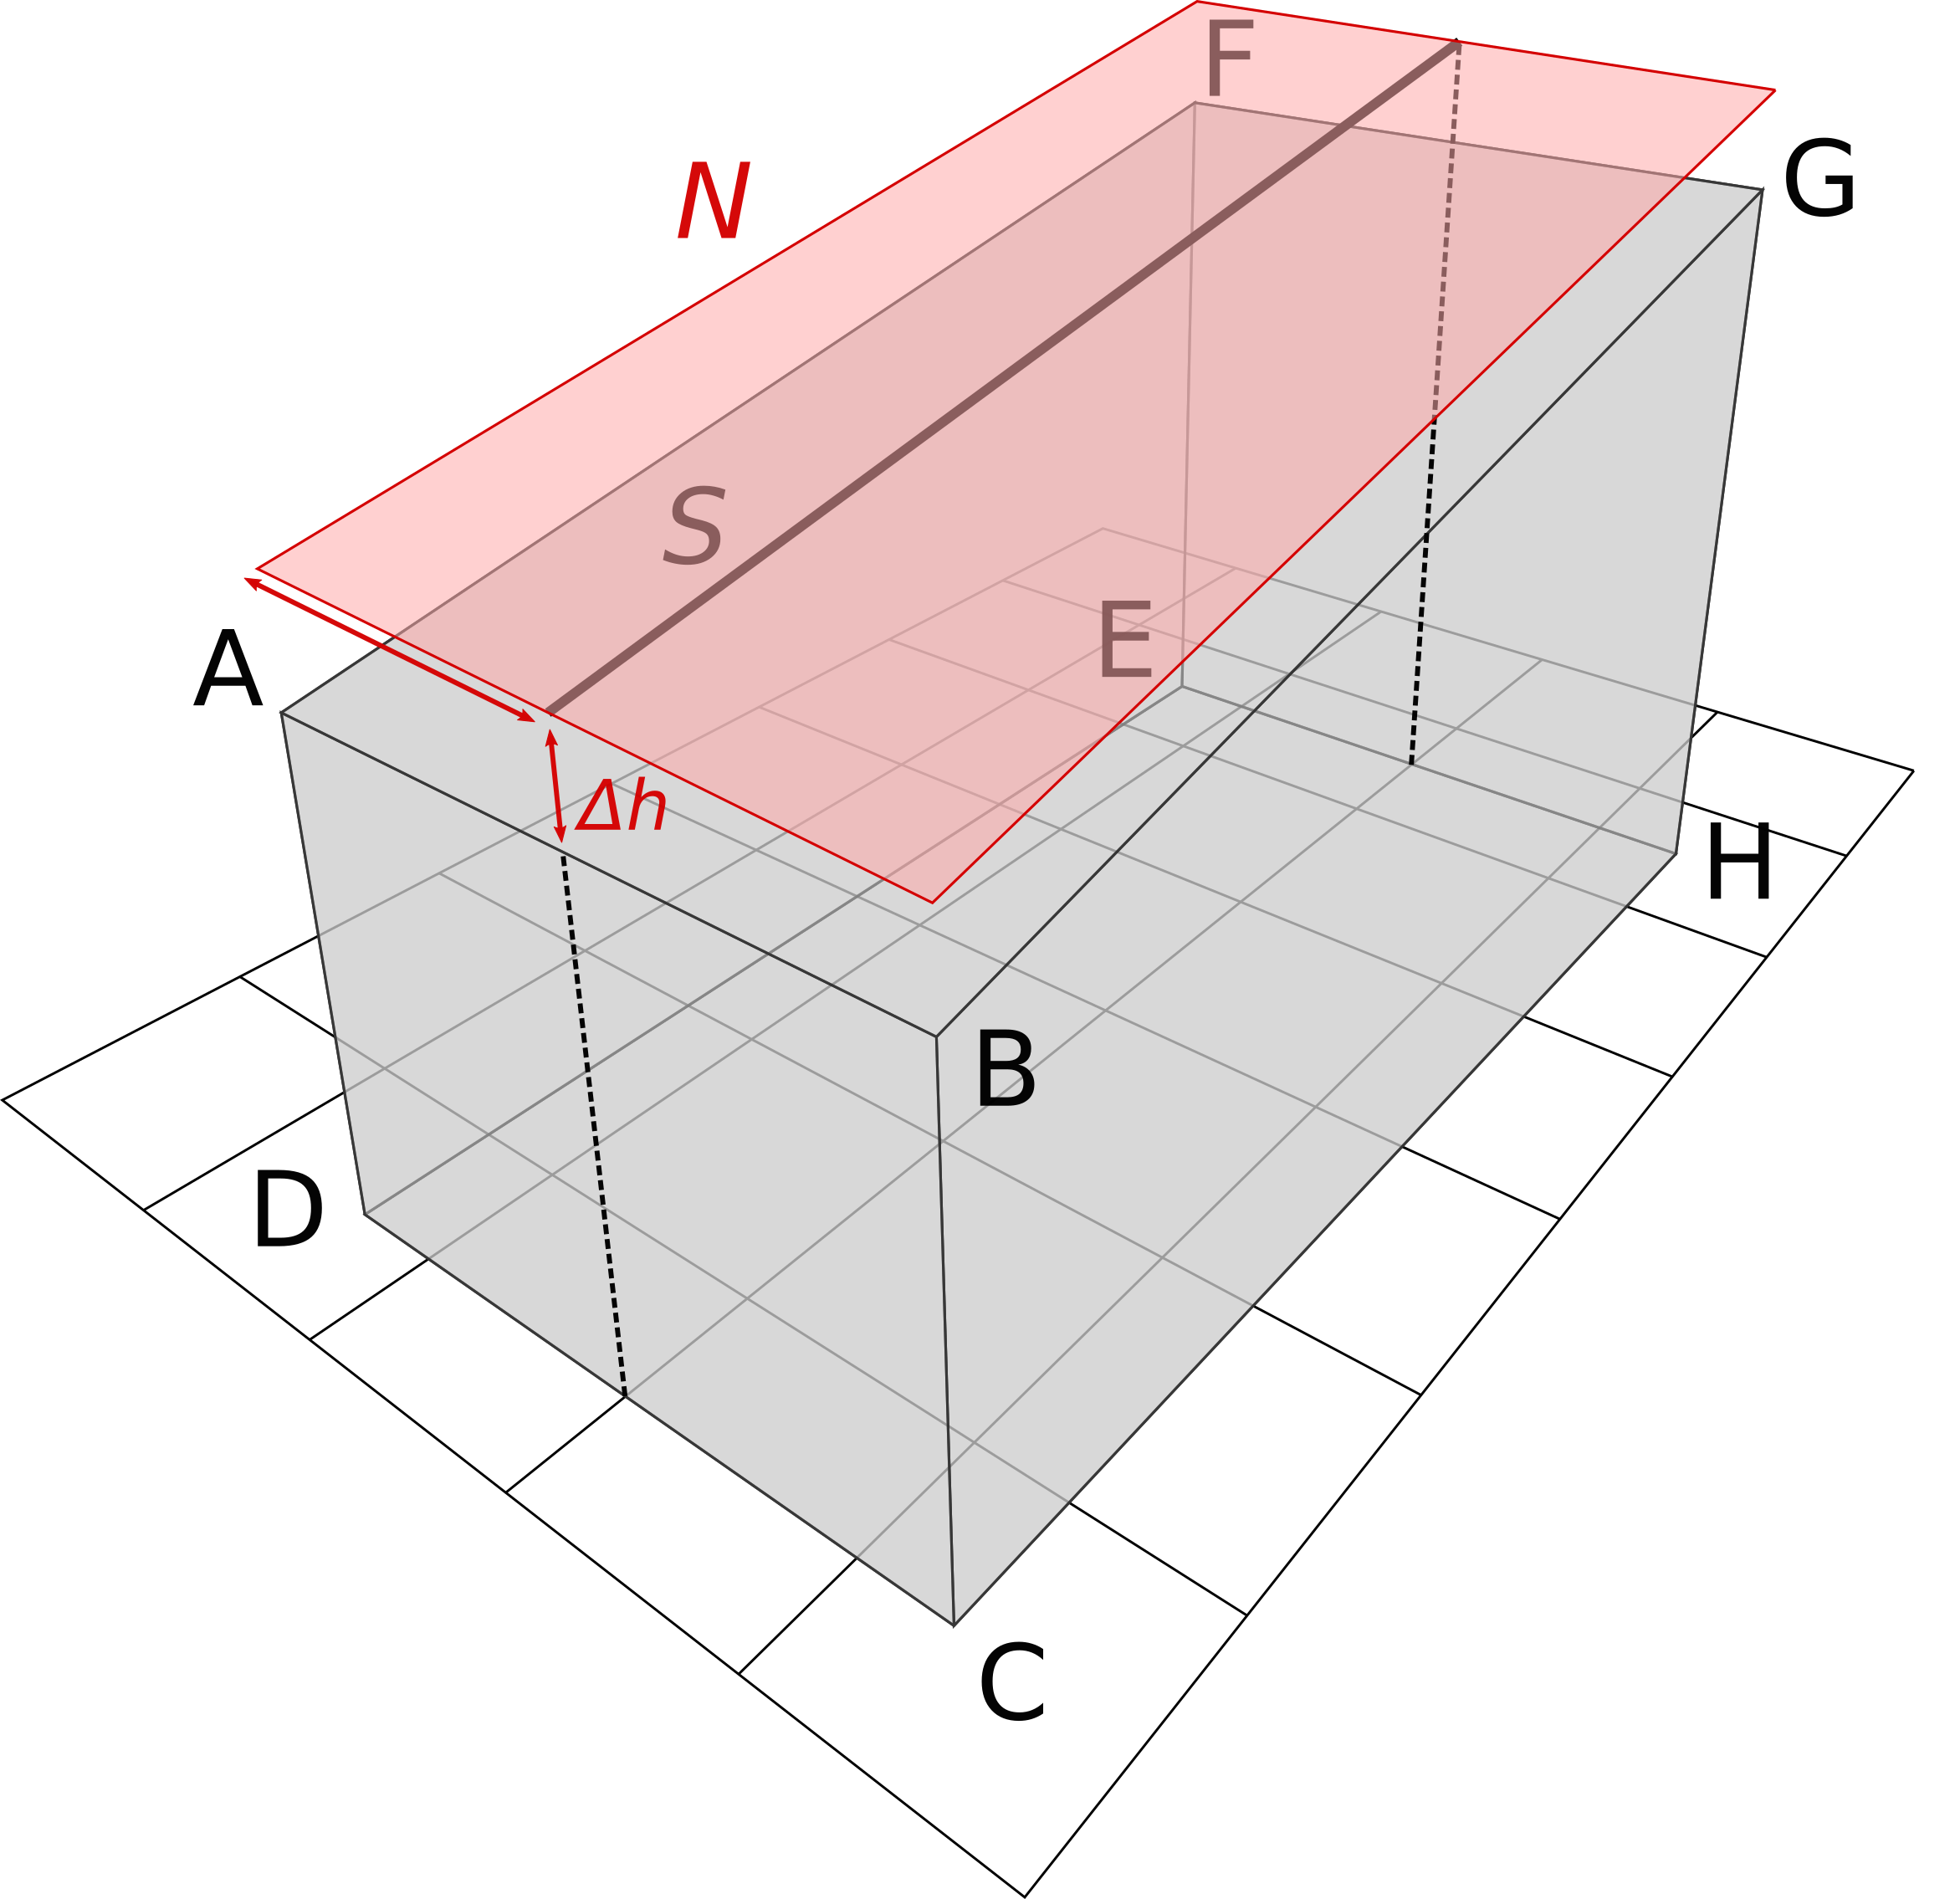
\includegraphics[height=0.3\textheight]{../figures/polyhedre.png}
  \caption{Plans utilisés pour définir une \emph{alpha-cut.}}
  \label{fig:schema_polyhedre}
\end{figure}

\begin{figure}
  \centering
  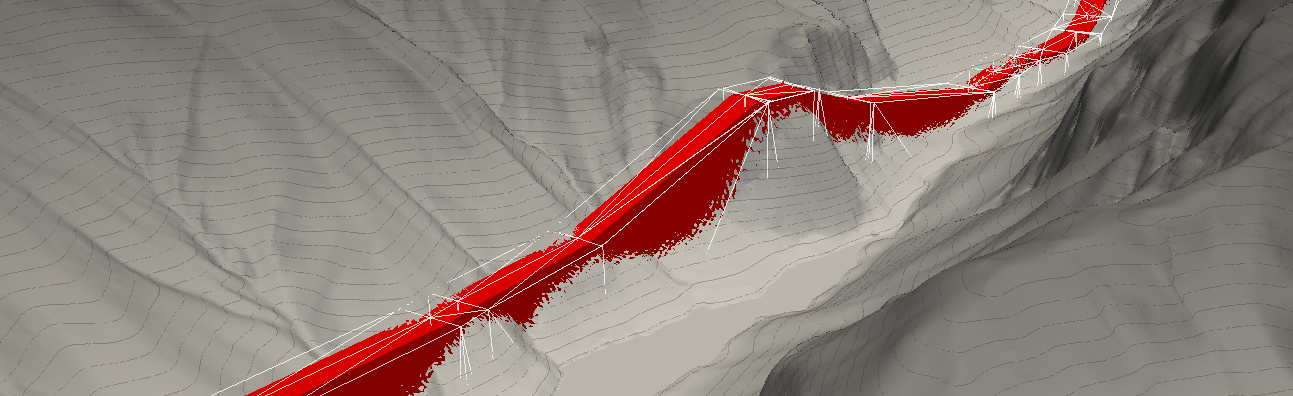
\includegraphics[width=\textwidth]{../figures/AlphaCut_coupe.png}
  \caption{Modélisation par \emph{alpha-cuts,} vue oblique.}
  \label{fig:AlphaCuts_coupe}
\end{figure}

\begin{figure}
  \centering
  \begin{tikzpicture}
  \tikzset{et/.style={above,font=\footnotesize\vphantom{Ag}}}
  % 
  \node[inner sep=0pt, anchor=south west] (image) at (0,0){\includegraphics{./figures/AlphaCut_zenith.png}};
  % 
  \begin{scope}
    \node (P2) at ([yshift=-.5cm]image.south east) {};
    \node (P1) at ([yshift=-.5cm]image.south west) {};

    \node (rect) [anchor=north west, minimum width=1cm,minimum
    height=.25cm] at ([yshift=-.25cm]P1) {}; \path[draw=RdBu-9-1, line
    width=.4mm](rect.west) --([xshift=-1ex]rect.south) -- ([xshift=1ex]rect.north)
    -- (rect.east);
    \node[anchor=west, font=\tiny\vphantom{Ag}, text width = 4cm] at
    ([xshift=1ex]rect.east) {Ligne électrique utilisée comme
      \emph{objet de référence}};

    \node (rect2) [anchor=north west, minimum width=1cm,minimum
    height=.25cm] at ([xshift=5.5cm,yshift=-.25cm]P1)
    {};

    \node[anchor=west, minimum width=.5cm,minimum
    height=.25cm, fill=RdBu-9-8] (rect2-1) at (rect2.west) {};

    \node[anchor=south west, minimum width=.5cm,minimum
    height=.25cm, fill=RdBu-9-9] (rect2-2) at (rect2-1.north west) {};
    
    \node[anchor=north west, minimum width=.5cm,minimum
    height=.25cm, fill=RdBu-9-7] (rect2-3) at (rect2-1.south west) {};

    \node[anchor=west, font=\fontsize{5}{5.5}\selectfont] at
    ([xshift=.5ex]rect2-1.east) {$0< \mu < 1$};
    
    \node[anchor=west, font=\fontsize{5}{5.5}\selectfont] at
    ([xshift=.5ex]rect2-2.east) {$\mu = 1$};
    
    \node[anchor=west, font=\fontsize{5}{5.5}\selectfont] at
    ([xshift=.5ex]rect2-3.east) {$\mu > 0$};

    \draw[decorate,decoration={brace}] ([xshift=7.5ex]rect2-2.north
    east) -- ([xshift=7.5ex]rect2-3.south east);
    
    \node[anchor=west, font=\tiny\vphantom{Ag}, text width = 4cm] at
    ([xshift=6ex]rect2.east) {\emph{Alpha-cuts} pour les valeurs du
      \emph{degré d'appartenance} ($\mu$) à la \ac{zlp}};

    % Échelle
    \draw[-] (P2 |- -1cm,-1cm) --++ (-1,0) node[et,pos=.5] {\SI{500}{\meter}};
    % Légende détaillée
    \path (P1) -- (P2) node[pos=.5, yshift=-1cm] {\tiny Pour la légende détaillée du fond topographique voir \autoref{anx:topo_leg}. Sources: BD TOPO 2018, BD ALTI 2018.}; 
  \end{scope}
\end{tikzpicture}
  %\includegraphics[width=\textwidth]{../figures/AlphaCut_zenith.png}
  \caption{Modélisation par \emph{alpha-cuts,} vue zénithale.}
  \label{fig:AlphaCuts_zenith}
\end{figure}

\subsection{Comparaison et choix de l'implémentation}

Bien que \emph{l'indice de localisation} utilisé pour la comparaison
soit relativement simple, il a permis de mettre en évidence des
différences assez conséquentes entre les approches raster et par
\emph{alpha-cuts.}

% Qualité de la modélisation
La qualité de la \emph{zone de localisation probable} créée est proche
avec les deux implémentations et nous n'avons repéré aucune différence
notable entre les deux \emph{zones de localisation probables}
\autocite{Bunel2019a}. Cependant, de part sa construction,
l'implémentation par \emph{alpha-cuts} devrait être, dans le cas
général, plus précise que l'approche raster, puisque ne nécessitant
pas un échantillonnage préalable. Toutefois, la précision de toutes
les implémentations dépend également de la précision des données. Par
exemple, la \emph{spatialisation} de la \emph{relation de
  localisation} \onto[orl]{Sous\-Pro\-che\-De} a nécessité l'emploi de
données altimétriques, diffusées sous la forme d'un \ac{mnt} de
résolution donnée. La spatialisation de la \emph{relation de
  localisation atomique}
\onto[orla]{Al\-ti\-tu\-de\-Stric\-te\-ment\-Inf\-érieu\-re} ne peut
donc pas, quelle que soit l'implémentation choisie, être plus précise
que la donnée en entrée. Or, comme l'implémentation raster a été
calculée à partir d'un raster dont la résolution est calquée sur celle
du \ac{mnt}, sa précision est identique à celle des données, dans
cette configuration l'implémentation par \emph{alpha-cuts} ne peut
donc pas être plus précise. Ainsi, la précision de l'ensemble de la
modélisation est avant tout limité par l'élément le moins précis, qui
dans le cas des deux implémentations est la précision du \ac{mnt}.

% \missingfigure{Différence zones}

% Difficulté de mise en place
Si les implémentations par \emph{alpha-cut} et raster proposent une
modélisation de qualité comparable, leur difficulté de mise en place
et de manipulation sont très différentes. La mise en place de ces deux
implémentations a nécessité des développements \emph{ad hoc.} Nous
n'avons pas éprouvé de difficulté particulière à mettre en place
l'implémentation raster, contrairement à l'approche par
\emph{alpha-cuts} qui a nécessité des développements conséquents et de
bas niveau. Si les problématiques techniques (\eg difficulté
d'implémentation, temps de calcul, \emph{etc.}) ne sont pas un critère
de décision suffisant, elles impliquent un investissement plus
important sur des tâches de développement, ce qui limite le temps
disponible pour l'implémentation de nouvelles méthodes de
\emph{spatialisation.} De plus, cela complique également l'extension
de la modélisation. L'ajout de nouvelles méthodes de
\emph{spatialisation} ou l'utilisation de nouveaux opérateurs flous
nécessiterait d'importants développements pour être utilisés avec
l'approche par \emph{alpha-cuts,} la méthode de construction du
polyèdre utilisée ne pouvant fonctionner qu'avec les \emph{relations
  de localisation atomiques}
\onto{Al\-ti\-tu\-de\-Stric\-te\-ment\-Inf\-érieu\-re} et
\onto[orla]{Dis\-tan\-ce\-Quan\-ti\-ta\-ti\-ve\-Pla\-ni\-mé\-tri\-que}
et les opérateurs de \textcite{Zadeh1965}. De plus, la généralisation
de l'utilisation de l'implémentation par \emph{alpha-cuts} nécessite
de compléter notre proposition pour offir une meilleure prise en
compte des jointures entre \emph{objets de référence,} toutes les
configurations ne permettant pas l'approximation fait ici.

% Tendance à la fragmentation des alpha-cuts
La généralisation de l'implémentation par \emph{alpha-cuts} impose
également de multiplier les étapes de \emph{fusion} \footnote{Seule la
  \emph{fusion} des \emph{zones de localisation compatibles} résultant
  de la \emph{spatialisation} des \emph{relations de localisation
    atomiques} (première étape de la phase de fusion,
  cf. \autoref{fig:methodo_1}) est ici prise en compte.} et donc les
intersections et unions entre \emph{alpha-cuts.} Si leur mise en place
n'est pas problématique, cela tend à complexifier les \emph{zones de
  localisations,} les \emph{alpha-cuts} devenant à chaque fusion plus
fragmentées et difficiles à interpréter visuellement, d'autant plus si
elles sont modélisées en trois dimensions. Le problème ne se pose pas
avec l'implémentation raster, puisque les intersections et les unions
sont réalisées au niveau des pixels. Le raster produit par ces
opérations est donc de forme identique à ceux intersectés. Ainsi,
alors que les \emph{alpha-cuts} tendent à ce complexifier à chaque
\emph{fusion,} les rasters restent similaires et donc de complexité
similaire.

% Temps de calcul
D'autres critères techniques peuvent également être pris en compte
pour cette comparaison, comme le temps de calcul nécessaire au
fonctionnement des deux implémentions ou le volume des données
qu'elles imposent de manipuler. Si l'on compare le temps nécessaire à
la construction des \emph{zones de localisations probables}
correspondant à \emph{l'indice de localisation} modélisé (Figures
\ref{fig:ZLP_SOUS_HT} et \ref{XX}), l'implémentation raster est plus
rapide. Mais cette performance est plus liée à des facteurs exogènes,
comme la qualité du développement et l'optimisation des bibliothèques
logicielles utilisées qu'a la complexité des algorithme utilisés. Par
exemple, l'implémentation par \emph{alpha-cuts} ayant été plus longue
et difficile à mettre en place, peu de temps a été consacré à
l'optimisation, même basique, de son code, ses performances sont donc
très certainement améliorables. De plus, le temps de calcul de
l'implémentation raster a tendance à augmenter plus rapidement avec le
nombre \emph{d'objets de référence} à traiter (ou avec la résolution
utilisée), cette méthode est donc potentiellement moins performante
que l'approche par \emph{alpha-cuts,} même si la spatialisation de
l'indice de localisation : \enquote{Je suis sous une ligne électrique
  trois brins} semble indiquer le contraire.

% Volume des données
L'implémentation par \emph{alpha-cut} a également l'avantage ---~cette
fois encore plus net~--- si l'on se penche sur la question du volume
des données produites et manipulées. Là où les \emph{alpha-cut} sont
construites directement, l'implémentation raster nécessite de
pré-calculer un raster par \emph{métriques} et par \emph{objet de
  référence} avant de pouvoir construire les \emph{zones de
  localisation compatibles.} Le nombre de raster peut augmenter
fortement avec le nombre \emph{d'objets de référence} ou
\emph{d'indices de localisation,} conformément au \emph{principe de
  décomposition}, et leur taille quadratiquement avec la
résolution. L'utilisation d'une implémentation raster respectant les
\emph{principes de modélisation} définis est donc assez contraignante
du point de vue des données à manipuler.

% Choix du raster
Ces différents éléments de comparaison (\autoref{tab:comp_implems})
nous ont conduit à privilégier l'implémentation raster. Bien que
potentiellement moins performante que l'implémentation par
\emph{alpha-cuts,} cette approche s'est révélée plus simple et rapide
à mettre en place. De plus les développements nécessaires à la
généralisation de la méthode (\eg changement d'opérateurs
d'intersection et d'union, ajout de nouvelles méthodes de
\emph{spatialisation,} \emph{etc.}) sont moins contraignants et moins
couteux. Le choix d'une implémentation raster nous permet donc
d'aboutir plus rapidement une à méthode générique et fonctionnelle, ce
qui nous permettra de nous concentrer sur question de la
\emph{spatialisation} (et donc de traiter plus d'alertes) et non sur
des problèmes technique de programmation.

% Impacts
Le choix de l'implémentation raster nécessite la définition préalable
d'une résolution de traitement, de laquelle dépendra, toutes choses
égales par ailleurs, la précision de la \emph{spatialisation,} mais
également le temps de calcul et le volume des résultats. Si cette
résolution peut être importante pour de petites \ac{zir}
\footnote{Comme la \emph{zone initiale de recherche} de \emph{l'indice
    de localisation} ici traité. Cette dernière étant suffisamment
  réduite pour que nous puissions travailler avec la résolution
  maximale, celle de la moins précise des données (en l’occurrence le
  \ac{mnt}).}, elle doit nécessairement être réduite lorsque la
\ac{zir} grandi \footnote{Plus de pixels sont alors a traiter.} ou
lorsque les \emph{indices de localisation} se multiplient ou se
complexifient \footnote{Plus de \emph{zones de localisation
    compatibles,} doivent être construites.}.

\begin{landscape}
  \begin{table}[H]
    \centering
    \begin{tabular}{L{.3\textheight}L{.3\textheight}L{.3\textheight}} \toprule
\multicolumn{1}{c}{\bfseries Critère comparatif} &
\multicolumn{1}{c}{\bfseries \emph{Alpha-cuts}} & \multicolumn{1}{c}{\bfseries
Raster} \\ \midrule
% Sémantique des relations spatiales
  Précision de la modélisation & Dépend avant tout de la précision des
                                 données. & Dépend avant tout de la
                                            résolution, puis de la précision
                                            des données.\\
  Difficulté de mise en place & Assez importante. La mise en place de
                                cette implémentation nécessite de nombreux
                                développements \emph{ad hoc} de bas
                                niveau & Peu importante. Il est assez
                                         rapide d'aboutir aux premières
                                         \emph{spatialisations.}\\
  %
  Difficulté d'extension & Importante ; il est difficile de
                           généraliser l'implémentation pour y
                           adjoindre de nouvelles méthodes de
                           \emph{spatialisation.}  &  Faible ; une
                                                     fois les
                                                     premières
                                                     \emph{spatialisations}
                                                     effectuées, peu
                                                     de modifications
                                                     sont à prévoir. \\
  %
  Temps de calcul & Assez faible pour l'exemple traité, risque
                    de varier fortement en fonction de la \emph{relation de
                    localisation} traitée. & Conséquent. Augmente quadratiquement avec la
                      résolution.\\
  %
  Volume des données & Assez faible. & Assez faible pour aboutir à la \autoref{fig:ZLP_SOUS_HT}, mais augmente rapidement avec le
                                       nombre \emph{d'objets de référence} candidats.\\
  %
  Contraintes spécifiques &Nécessité de choisir le nombre et le degré
                            d'appartenance des \emph{alpha-cuts.} & Nécessité de définir une résolution de modélisation.\\
  \bottomrule
\end{tabular}

    \caption{Synthèse de la comparaison des implémentations par
      \emph{alpha-cuts} et raster.}
    \label{tab:comp_implems}
  \end{table}
\end{landscape}

%%% Local Variables:
%%% mode: latex
%%% TeX-master: "../../../../main"
%%% End:
